\documentclass{beamer}

\setbeamertemplate{navigation symbols}{}
\setbeamertemplate{footline}[frame number]

\usepackage{amsfonts}
\usepackage{amsmath}
\usepackage{amssymb}
\usepackage{amsthm}
\usepackage{caption}

\usepackage{tikz}
\usetikzlibrary{graphs}

\usepackage[indent=0pt]{parskip}

\usepackage{natbib}

\bibliographystyle{abbrvnat}
\setcitestyle{authoryear,open={(},close={)}} %Citation-related commands

%\newtheorem{theorem}{Theorem}[section]
%\newtheorem{lemma}[theorem]{Lemma}

%Information to be included in the title page:
\title{Burning Spiders}
\subtitle{AM8204 - Topics in Discrete Mathematics}
\author{Ryan DeWolfe}
\institute{Toronto Metropolitan University}
\date{April 2025}

\begin{document}

\begin{frame}[plain]
    \titlepage
   \end{frame}

\begin{frame}{Motivation}
\begin{itemize}
\item The burning number conjecture is true if it true for trees.
\item Spiders are a subset of trees.
\item We are following a proof from the paper
\end{itemize}
\hspace{0.7cm} A. Bonato and T. Lidbetter. Bounds on the burning\\
\hspace{0.7cm} numbers of spiders and path-forests. \textit{Theoretical \\
\hspace{0.7cm} Computer Science}, 794:12-19, 2019.
\end{frame}

\begin{frame}{Preliminaries}
\begin{itemize}
\item A tree is a \textit{spider} if it has exactly one vertex with degree strictly greater than $3$.
\item The unique vertex with degree strictly greater than $3$ is called the \textit{head} and is denoted $h$.
\end{itemize}
\vspace{2em}
\begin{figure}
\centering
\begin{tiny}
    \hfill
    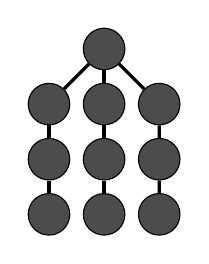
\begin{tikzpicture}[scale=0.7]
        \begin{scope}[every node/.style={fill=black!70,circle,draw=black, minimum size=1.5em}]
            \node (1) at (0,0) {};
            \node (2) at (1,0) {};
            \node (3) at (2,0) {};

            \node (4) at (0,1) {};
            \node (5) at (1,1) {};
            \node (6) at (2,1) {};

            \node (7) at (0,2) {};
            \node (8) at (1,2) {};
            \node (9) at (2,2) {};

            \node (10) at (1,3) {};
        \end{scope}
        \begin{scope}[every edge/.style={draw,very thick}]
            \path [-] (1) edge node {} (4);
            \path [-] (4) edge node {} (7);
            \path [-] (7) edge node {} (10);

            \path [-] (2) edge node {} (5);
            \path [-] (5) edge node {} (8);
            \path [-] (8) edge node {} (10);

            \path [-] (3) edge node {} (6);
            \path [-] (6) edge node {} (9);
            \path [-] (9) edge node {} (10);
        \end{scope}
    \end{tikzpicture}
    \hfill
    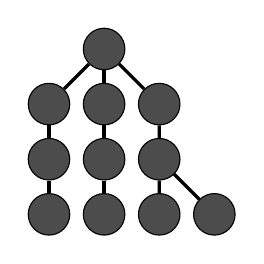
\begin{tikzpicture}[scale=0.7]
        \begin{scope}[every node/.style={fill=black!70,circle,draw=black, minimum size=1.5em}]
            \node (1) at (0,0) {};
            \node (2) at (1,0) {};
            \node (3) at (2,0) {};

            \node (4) at (0,1) {};
            \node (5) at (1,1) {};
            \node (6) at (2,1) {};

            \node (7) at (0,2) {};
            \node (8) at (1,2) {};
            \node (9) at (2,2) {};

            \node (10) at (1,3) {};
            
            \node (11) at (3, 0) {};
        \end{scope}
        \begin{scope}[every edge/.style={draw,very thick}]
            \path [-] (1) edge node {} (4);
            \path [-] (4) edge node {} (7);
            \path [-] (7) edge node {} (10);

            \path [-] (2) edge node {} (5);
            \path [-] (5) edge node {} (8);
            \path [-] (8) edge node {} (10);

            \path [-] (3) edge node {} (6);
            \path [-] (6) edge node {} (9);
            \path [-] (9) edge node {} (10);

            \path [-] (6) edge node {} (11);
        \end{scope}
    \end{tikzpicture}
    \hfill
    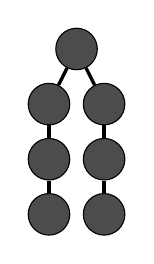
\begin{tikzpicture}[scale=0.7]
        \begin{scope}[every node/.style={fill=black!70,circle,draw=black, minimum size=1.5em}]
            \node (1) at (0,0) {};
            \node (2) at (1,0) {};

            \node (4) at (0,1) {};
            \node (5) at (1,1) {};

            \node (7) at (0,2) {};
            \node (8) at (1,2) {};
    
            \node (10) at (0.5,3) {};
        \end{scope}
        \begin{scope}[every edge/.style={draw,very thick}]
            \path [-] (1) edge node {} (4);
            \path [-] (4) edge node {} (7);
            \path [-] (7) edge node {} (10);

            \path [-] (2) edge node {} (5);
            \path [-] (5) edge node {} (8);
            \path [-] (8) edge node {} (10);
        \end{scope} 
    \end{tikzpicture}
    \hfill
\end{tiny}
\end{figure}
\hspace{5em} Yes \hspace{6em} No \hspace{7em} No

\end{frame}

\begin{frame}{Preliminaries}
    \begin{lemma}[Leftover Lemma]
        Let $G$ be a graph and $v \in V(G)$. Let $k$ a positive integer.
        If $b(G - N_{k-1}[v]) \leq k - 1$ then $b(G) \leq k$.
    \end{lemma}

    This lemma is used in an inductive step in the proofs of the following lemmas and is used often in the main theorem.
\end{frame}

\begin{frame}{Preliminaries}
    \begin{lemma}[Path-Forest Lemma]
        If $G$ is a path-forest with $t$ components then $b(G) \leq \lfloor \frac{n(G)}{2t} \rfloor + t$.
    \end{lemma}
\end{frame}

\begin{frame}{Preliminaries}
    \begin{lemma}[Graph Family Lemma]
        Let $\mathcal{G}$ be a set of connected graphs.
        Let $\hat{\mathcal{G}} \subseteq G$ with the following condition.
        For every $G \in \hat{\mathcal{G}}$, there exists $v \in V(G)$ and $r \leq \lceil \sqrt{n(G)}\ \rceil - 1$ such that at least one of the followng conditions are satisfied.
        \begin{enumerate}
            \item $N_r[v] = V(G).$
            \item $|N_r[v]| \geq 2\lceil \sqrt{n(G)}\ \rceil - 1$ and the induced subgraph\\ $G[V(G) \setminus N_r[v]]$ is in  $\mathcal{G}$.
        \end{enumerate}
        If $b(G) \leq \lceil \sqrt{n(G)}\ \rceil$ for all $G \in \mathcal{G} \backslash \hat{\mathcal{G}}$, then $b(G) \leq \lceil \sqrt{n(G)}\ \rceil$ for all $G \in \mathcal{G}$.
    \end{lemma}
\end{frame}

\begin{frame}{Main Theorem}
    \begin{theorem}[Theorem 7 in Bonato and Lidbetter (2019)]
        If $G$ is a spider then $b(G) \leq \lceil \sqrt{n(G)}\ \rceil$.
    \end{theorem}
\end{frame}

\begin{frame}{Proof of Main Theorem}
    Let $\alpha = \lceil \sqrt{n(G)} \rceil$.
    The proof procedes as follows:
    \begin{enumerate}
        \item Check all spides with at most $25$ vertices.
        \item Show the bound holds for spiders with a long arm(s) if it hold for spiders with short arms.
        \item Remove $N_{\alpha[h]}$ and argue the remaining path-forest can be burned in $\alpha - 1$ rounds.
    \end{enumerate}
\end{frame}

\begin{frame}{Check all spiders with at most $25$ vertices.}
\begin{itemize}
\item If $\sqrt{n(G)}$ is not an integer, then $G$ is a subgraph of a spider $H$ with $n(H) = \alpha^2$.\\
\item Given a burning sequence for $H$ we can construct a burning sequence for $G$ by "sliding" the neighborhoods up the arms (if necessary).
\end{itemize}
\end{frame}

\begin{frame}{Check all spiders with at most $25$ vertices.}
\begin{itemize}
\item If $n(G)=4$ there is only one spider and it can be burned in $2$ round by choosing the head in round $1$.
\item Suppose $n(G) = 9$.
\item If $G$ has an arm longer than $5$, that arm can be used as a neighborhood for the Graph Family lemma, and we take the family to include smaller spiders.
\item If $G - N_2[h]$ cannot have more than $2$ components or else it would need at least $10$ vertices.
\item If $G - N_2[h]$ has $1$ or $2$ compoents Path-Forest Lemma applies.
\end{itemize}
\end{frame}

\begin{frame}{Check all spiders with at most $25$ vertices.}
\begin{itemize}
    \item Applying the same arguments as the $n(G) = 9$ case when $n(G) = 16$ covers all spiders except those with $3$ arms with length at least $4$ and at most $6$.
\end{itemize}
\begin{figure}
    \centering
    \begin{tiny}
    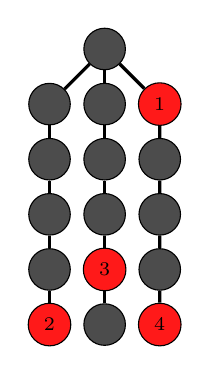
\begin{tikzpicture}[scale=0.7]
        \begin{scope}[every node/.style={fill=black!70,circle,draw=black, minimum size=1.5em}]
            \node[fill=red!90] (1) at (0,0) {\scriptsize 2};
            \node (2) at (1,0) {\:};
            \node[fill=red!90] (3) at (2,0) {\scriptsize 4};

            \node (4) at (0,1) {};
            \node[fill=red!90] (5) at (1,1) {\scriptsize 3};
            \node (6) at (2,1) {};

            \node (7) at (0,2) {};
            \node (8) at (1,2) {};
            \node (9) at (2,2) {};

            \node (10) at (0,3) {};
            \node (11) at (1,3) {};
            \node (12) at (2,3) {};

            \node (13) at (0,4) {};
            \node (14) at (1,4) {};
            \node (15)[fill=red!90] at (2,4) {\scriptsize 1};

            \node (16) at (1,5) {};
        \end{scope}
        \begin{scope}[every edge/.style={draw,very thick}]
            \path [-] (1) edge node {} (4);
            \path [-] (4) edge node {} (7);
            \path [-] (7) edge node {} (10);
            \path [-] (10) edge node {} (13);
            \path [-] (13) edge node {} (16);

            \path [-] (2) edge node {} (5);
            \path [-] (5) edge node {} (8);
            \path [-] (8) edge node {} (11);
            \path [-] (11) edge node {} (14);
            \path [-] (14) edge node {} (16);

            \path [-] (3) edge node {} (6);
            \path [-] (6) edge node {} (9);
            \path [-] (9) edge node {} (12);
            \path [-] (12) edge node {} (15);
            \path [-] (15) edge node {} (16);
        \end{scope}
    \end{tikzpicture}
    \hspace{2cm}
    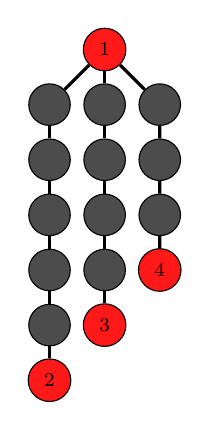
\begin{tikzpicture}[scale=0.7]
        \begin{scope}[every node/.style={fill=black!70,circle,draw=black, minimum size=1.5em}]
            \node (1) at (0,0) {};
            \node[fill=red!90] (2) at (1,0) {\scriptsize 3};
            \node[fill=red!90] (3) at (0,-1) {\scriptsize 2};

            \node (4) at (0,1) {};
            \node (5) at (1,1) {};
            \node[fill=red!90] (6) at (2,1) {\scriptsize 4};

            \node (7) at (0,2) {};
            \node (8) at (1,2) {};
            \node (9) at (2,2) {};

            \node (10) at (0,3) {};
            \node (11) at (1,3) {};
            \node (12) at (2,3) {};

            \node (13) at (0,4) {};
            \node (14) at (1,4) {};
            \node (15) at (2,4) {};

            \node[fill=red!90] (16) at (1,5) {\scriptsize 1};
        \end{scope}
        \begin{scope}[every edge/.style={draw,very thick}]
            \path [-] (1) edge node {} (4);
            \path [-] (4) edge node {} (7);
            \path [-] (7) edge node {} (10);
            \path [-] (10) edge node {} (13);
            \path [-] (13) edge node {} (16);

            \path [-] (2) edge node {} (5);
            \path [-] (5) edge node {} (8);
            \path [-] (8) edge node {} (11);
            \path [-] (11) edge node {} (14);
            \path [-] (14) edge node {} (16);

            \path [-] (3) edge node {} (1);
            \path [-] (6) edge node {} (9);
            \path [-] (9) edge node {} (12);
            \path [-] (12) edge node {} (15);
            \path [-] (15) edge node {} (16);
        \end{scope}
    \end{tikzpicture}
    \end{tiny}
\end{figure}
\end{frame}

\begin{frame}{Check all spiders with at most $25$ vertices.}
\begin{itemize}
\item The same argument when $n(G) = 25$ covers all cases except for at least $3$ arms with lengths at least $5$ and at most $8$.
\item If there are $3$ arms, $G-N_4[h]$ must have $12$ vertices, and if there are $4$ arms $G-N_4[h]$ must have $8$ vertices.
\end{itemize}
\begin{figure}
    \begin{tiny}
    \centering
    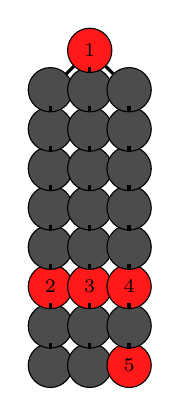
\begin{tikzpicture}[scale=0.5]
        \begin{scope}[every node/.style={fill=black!70,circle,draw=black, minimum size=1.6em}]
            \node (1) at (0,0) {};
            \node (2) at (1,0) {};
            \node[fill=red!90] (3) at (2,0) {\scriptsize 5};

            \node (4) at (0,1) {};
            \node (5) at (1,1) {};
            \node (6) at (2,1) {};

            \node[fill=red!90] (7) at (0,2) {\scriptsize 2};
            \node[fill=red!90] (8) at (1,2) {\scriptsize 3};
            \node[fill=red!90] (9) at (2,2) {\scriptsize 4};

            \node (10) at (0,3) {};
            \node (11) at (1,3) {};
            \node (12) at (2,3) {};

            \node (13) at (0,4) {};
            \node (14) at (1,4) {};
            \node (15) at (2,4) {};

            \node (16) at (0,5) {};
            \node (17) at (1,5) {};
            \node (18) at (2,5) {};

            \node (19) at (0,6) {};
            \node (20) at (1,6) {};
            \node (21) at (2,6) {};

            \node (22) at (0,7) {};
            \node (23) at (1,7) {};
            \node (24) at (2,7) {};

            \node[fill=red!90] (25) at (1,8) {\scriptsize 1};
        \end{scope}
        \begin{scope}[every edge/.style={draw,very thick}]
            \path [-] (1) edge node {} (4);
            \path [-] (4) edge node {} (7);
            \path [-] (7) edge node {} (10);
            \path [-] (10) edge node {} (13);
            \path [-] (13) edge node {} (16);
            \path [-] (16) edge node {} (19);
            \path [-] (19) edge node {} (22);
            \path [-] (22) edge node {} (25);

            \path [-] (2) edge node {} (5);
            \path [-] (5) edge node {} (8);
            \path [-] (8) edge node {} (11);
            \path [-] (11) edge node {} (14);
            \path [-] (14) edge node {} (17);
            \path [-] (17) edge node {} (20);
            \path [-] (20) edge node {} (23);
            \path [-] (23) edge node {} (25);

            \path [-] (3) edge node {} (6);
            \path [-] (6) edge node {} (9);
            \path [-] (9) edge node {} (12);
            \path [-] (12) edge node {} (15);
            \path [-] (15) edge node {} (18);
            \path [-] (18) edge node {} (21);
            \path [-] (21) edge node {} (24);
            \path [-] (24) edge node {} (25);
        \end{scope}
    \end{tikzpicture}
    \hfill
    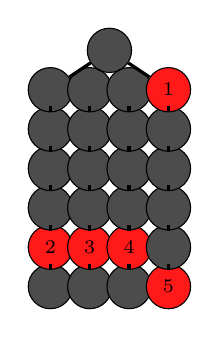
\begin{tikzpicture}[scale=0.5]
        \begin{scope}[every node/.style={fill=black!70,circle,draw=black, minimum size=1.6em}]
            \node (1) at (0,0) {};
            \node (2) at (1,0) {};
            \node (3) at (2,0) {};
            \node[fill=red!90] (4) at (3,0) {\scriptsize 5};

            \node[fill=red!90] (5) at (0,1) {\scriptsize 2};
            \node[fill=red!90] (6) at (1,1) {\scriptsize 3};
            \node[fill=red!90] (7) at (2,1) {\scriptsize 4};
            \node (8) at (3,1) {};

            \node (9) at (0,2) {};
            \node (10) at (1,2) {};
            \node (11) at (2,2) {};
            \node (12) at (3,2) {};

            \node (13) at (0,3) {};
            \node (14) at (1,3) {};
            \node (15) at (2,3) {};
            \node (16) at (3,3) {};

            \node (17) at (0,4) {};
            \node (18) at (1,4) {};
            \node (19) at (2,4) {};
            \node (20) at (3,4) {};

            \node (21) at (0,5) {};
            \node (22) at (1,5) {};
            \node (23) at (2,5) {};
            \node[fill=red!90] (24) at (3,5) {\scriptsize 1};

            \node (25) at (1.5,6) {};
        \end{scope}
        \begin{scope}[every edge/.style={draw,very thick}]
            \path [-] (1) edge node {} (5);
            \path [-] (5) edge node {} (9);
            \path [-] (9) edge node {} (13);
            \path [-] (13) edge node {} (17);
            \path [-] (17) edge node {} (21);
            \path [-] (21) edge node {} (25);

            \path [-] (2) edge node {} (6);
            \path [-] (6) edge node {} (10);
            \path [-] (10) edge node {} (14);
            \path [-] (14) edge node {} (18);
            \path [-] (18) edge node {} (22);
            \path [-] (22) edge node {} (25);

            \path [-] (3) edge node {} (7);
            \path [-] (7) edge node {} (11);
            \path [-] (11) edge node {} (15);
            \path [-] (15) edge node {} (19);
            \path [-] (19) edge node {} (23);
            \path [-] (23) edge node {} (25);

            \path [-] (4) edge node {} (8);
            \path [-] (8) edge node {} (12);
            \path [-] (12) edge node {} (16);
            \path [-] (16) edge node {} (20);
            \path [-] (20) edge node {} (24);
            \path [-] (24) edge node {} (25);
        \end{scope}
    \end{tikzpicture}
    \hfill
    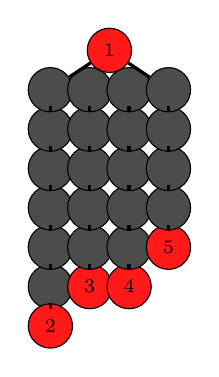
\begin{tikzpicture}[scale=0.5]
        \begin{scope}[every node/.style={fill=black!70,circle,draw=black, minimum size=1.6em}]
            \node (1) at (0,0) {};
            \node[fill=red!90] (2) at (1,0) {\scriptsize 3};
            \node[fill=red!90] (3) at (2,0) {\scriptsize 4};
            \node[fill=red!90] (4) at (0,-1) {\scriptsize 2};

            \node (5) at (0,1) {};
            \node (6) at (1,1) {};
            \node (7) at (2,1) {};
            \node[fill=red!90] (8) at (3,1) {\scriptsize 5};

            \node (9) at (0,2) {};
            \node (10) at (1,2) {};
            \node (11) at (2,2) {};
            \node (12) at (3,2) {};

            \node (13) at (0,3) {};
            \node (14) at (1,3) {};
            \node (15) at (2,3) {};
            \node (16) at (3,3) {};

            \node (17) at (0,4) {};
            \node (18) at (1,4) {};
            \node (19) at (2,4) {};
            \node (20) at (3,4) {};

            \node (21) at (0,5) {};
            \node (22) at (1,5) {};
            \node (23) at (2,5) {};
            \node (24) at (3,5) {};

            \node[fill=red!90] (25) at (1.5,6) {\scriptsize 1};
        \end{scope}
        \begin{scope}[every edge/.style={draw,very thick}]
            \path [-] (1) edge node {} (5);
            \path [-] (5) edge node {} (9);
            \path [-] (9) edge node {} (13);
            \path [-] (13) edge node {} (17);
            \path [-] (17) edge node {} (21);
            \path [-] (21) edge node {} (25);

            \path [-] (2) edge node {} (6);
            \path [-] (6) edge node {} (10);
            \path [-] (10) edge node {} (14);
            \path [-] (14) edge node {} (18);
            \path [-] (18) edge node {} (22);
            \path [-] (22) edge node {} (25);

            \path [-] (3) edge node {} (7);
            \path [-] (7) edge node {} (11);
            \path [-] (11) edge node {} (15);
            \path [-] (15) edge node {} (19);
            \path [-] (19) edge node {} (23);
            \path [-] (23) edge node {} (25);

            \path [-] (4) edge node {} (1);
            \path [-] (8) edge node {} (12);
            \path [-] (12) edge node {} (16);
            \path [-] (16) edge node {} (20);
            \path [-] (20) edge node {} (24);
            \path [-] (24) edge node {} (25);
        \end{scope}
    \end{tikzpicture}
    \hfill
    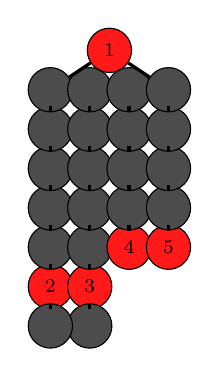
\begin{tikzpicture}[scale=0.5]
        \begin{scope}[every node/.style={fill=black!70,circle,draw=black, minimum size=1.6em}]
            \node[fill=red!90] (1) at (0,0) {\scriptsize 2};
            \node[fill=red!90] (2) at (1,0) {\scriptsize 3};
            \node (3) at (1,-1) {};
            \node (4) at (0,-1) {};

            \node (5) at (0,1) {};
            \node (6) at (1,1) {};
            \node[fill=red!90] (7) at (2,1) {\scriptsize 4};
            \node[fill=red!90] (8) at (3,1) {\scriptsize 5};

            \node (9) at (0,2) {};
            \node (10) at (1,2) {};
            \node (11) at (2,2) {};
            \node (12) at (3,2) {};

            \node (13) at (0,3) {};
            \node (14) at (1,3) {};
            \node (15) at (2,3) {};
            \node (16) at (3,3) {};

            \node (17) at (0,4) {};
            \node (18) at (1,4) {};
            \node (19) at (2,4) {};
            \node (20) at (3,4) {};

            \node (21) at (0,5) {};
            \node (22) at (1,5) {};
            \node (23) at (2,5) {};
            \node (24) at (3,5) {};

            \node[fill=red!90] (25) at (1.5,6) {\scriptsize 1};
        \end{scope}
        \begin{scope}[every edge/.style={draw,very thick}]
            \path [-] (1) edge node {} (5);
            \path [-] (5) edge node {} (9);
            \path [-] (9) edge node {} (13);
            \path [-] (13) edge node {} (17);
            \path [-] (17) edge node {} (21);
            \path [-] (21) edge node {} (25);

            \path [-] (2) edge node {} (6);
            \path [-] (6) edge node {} (10);
            \path [-] (10) edge node {} (14);
            \path [-] (14) edge node {} (18);
            \path [-] (18) edge node {} (22);
            \path [-] (22) edge node {} (25);

            \path [-] (3) edge node {} (2);
            \path [-] (7) edge node {} (11);
            \path [-] (11) edge node {} (15);
            \path [-] (15) edge node {} (19);
            \path [-] (19) edge node {} (23);
            \path [-] (23) edge node {} (25);

            \path [-] (4) edge node {} (1);
            \path [-] (8) edge node {} (12);
            \path [-] (12) edge node {} (16);
            \path [-] (16) edge node {} (20);
            \path [-] (20) edge node {} (24);
            \path [-] (24) edge node {} (25);
        \end{scope}
    \end{tikzpicture}
    \hfill
    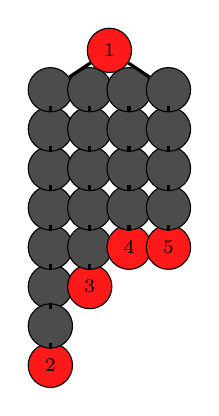
\begin{tikzpicture}[scale=0.5]
        \begin{scope}[every node/.style={fill=black!70,circle,draw=black, minimum size=1.6em}]
            \node (1) at (0,0) {};
            \node[fill=red!90] (2) at (1,0) {\scriptsize 3};
            \node[fill=red!90] (3) at (0,-2) {\scriptsize 2};
            \node (4) at (0,-1) {};

            \node (5) at (0,1) {};
            \node (6) at (1,1) {};
            \node[fill=red!90] (7) at (2,1) {\scriptsize 4};
            \node[fill=red!90] (8) at (3,1) {\scriptsize 5};

            \node (9) at (0,2) {};
            \node (10) at (1,2) {};
            \node (11) at (2,2) {};
            \node (12) at (3,2) {};

            \node (13) at (0,3) {};
            \node (14) at (1,3) {};
            \node (15) at (2,3) {};
            \node (16) at (3,3) {};

            \node (17) at (0,4) {};
            \node (18) at (1,4) {};
            \node (19) at (2,4) {};
            \node (20) at (3,4) {};

            \node (21) at (0,5) {};
            \node (22) at (1,5) {};
            \node (23) at (2,5) {};
            \node (24) at (3,5) {};

            \node[fill=red!90] (25) at (1.5,6) {\scriptsize 1};
        \end{scope}
        \begin{scope}[every edge/.style={draw,very thick}]
            \path [-] (1) edge node {} (5);
            \path [-] (5) edge node {} (9);
            \path [-] (9) edge node {} (13);
            \path [-] (13) edge node {} (17);
            \path [-] (17) edge node {} (21);
            \path [-] (21) edge node {} (25);

            \path [-] (2) edge node {} (6);
            \path [-] (6) edge node {} (10);
            \path [-] (10) edge node {} (14);
            \path [-] (14) edge node {} (18);
            \path [-] (18) edge node {} (22);
            \path [-] (22) edge node {} (25);

            \path [-] (3) edge node {} (4);
            \path [-] (7) edge node {} (11);
            \path [-] (11) edge node {} (15);
            \path [-] (15) edge node {} (19);
            \path [-] (19) edge node {} (23);
            \path [-] (23) edge node {} (25);

            \path [-] (4) edge node {} (1);
            \path [-] (8) edge node {} (12);
            \path [-] (12) edge node {} (16);
            \path [-] (16) edge node {} (20);
            \path [-] (20) edge node {} (24);
            \path [-] (24) edge node {} (25);
        \end{scope}
    \end{tikzpicture}
    \end{tiny}
\end{figure}
\end{frame}

\begin{frame}{Long Arms}
\begin{itemize}
\item If one arm of $G$ has length $\ell > 2\alpha - 2$, then there is a neighborhood on that arm to satisfy the Graph Family Lemma.
\item $|N_{\lceil \ell \slash 2 \rceil}[v]| = 2(\lceil \frac{\ell}{2}\rceil) + 1 \geq 2\alpha - 1$ for vertex $v$ that is distance $\lceil \frac{\ell}{2} \rceil$ from the end of the arm.
\item We can inductively remove a long arm until we are left with $n(G) \leq 25$ or no long arms.
\end{itemize}
\end{frame}

\begin{frame}{Remove $N_\alpha[h]$}
\begin{itemize}
\item Let $G' = G - N_{\alpha}[h]$.
\item $G'$ is a path forest whose components have length at most $\alpha - 1$.
\item If there are $ \leq \frac{\alpha}{2}$ components, then each component can be covered by a neighborhood of size $\alpha - i$, $1 \leq i \leq t$.
\item If $\alpha$ is odd, and $t = \frac{\alpha + 1}{2}$, the $t$th compnent can be covered with neighborhood of size $\frac{\alpha - 1}{2}$ and $1$.
\end{itemize}
\end{frame}

\begin{frame}{Remove $N_\alpha[h]$}
\begin{itemize}
\item So, $t \geq \lfloor \frac{\alpha + 1}{2} \rfloor + 1$.
\item Since at least $\alpha - 1$ arms got removed for each compnent in $G'$:
\end{itemize}
\begin{align*}
    n(G')&= n(G) - |N_{\alpha - 1}[h]|\\
    &\leq n(G) - (t(\alpha - 1) + 1)\\
    &\leq (\alpha - 1)(\alpha + 1 - t).
\end{align*}
\end{frame}

\begin{frame}{Remove $N_\alpha[h]$}
    $$n(G') \leq (\alpha - 1)(\alpha + 1 - t)$$
\begin{itemize}
\item Since $n(G') > 0$, $t < \alpha + 1$.
\item Since $n(G') \geq t$, $t \neq \alpha$.
\item If $t = \alpha - 1$ we can apply the Path-Forest Lemma to $G$.
\item So $\lfloor \frac{\alpha}{2} \rfloor + 1 \leq t \leq \alpha - 2$.
\end{itemize}
\end{frame}

\begin{frame}{Remove $N_\alpha[h]$}
\begin{itemize}
\item From the Path-Forest Lemma,
\begin{align*}
    b(G') \leq& \left\lfloor \frac{n(G')}{2t} \right\rfloor + t\\
    \leq& \lfloor \frac{\alpha^2 - 1}{2t} - \frac{\alpha - 1}{2} \rfloor + t
\end{align*}
\item We treat this as a real valued function and maximize, the maximum is at an endpoint of the interval.
\item Both endpoints are bounded above by $\alpha - 1$.
\item So, $b(G') \leq \alpha - 1$ and we apply the Leftover Lemma.
\end{itemize}
\end{frame}

\begin{frame}{Conclusion}
\begin{itemize}
\item We showed that spiders satisfy the burning number conjecture.
\item The proof was originally published in the following paper:
\end{itemize}
\hspace{0.7cm} A. Bonato and T. Lidbetter. Bounds on the burning\\
\hspace{0.7cm} numbers of spiders and path-forests. \textit{Theoretical \\
\hspace{0.7cm} Computer Science}, 794:12-19, 2019.
\end{frame}

\end{document}